\documentclass[handout]{beamer}

\usepackage[utf8]{inputenc}
\usepackage[frenchb]{babel}
\usepackage{verbatim}
\usepackage{graphicx}
\usepackage{color}
\usepackage{hyperref}
\usepackage{verbatim}
\usepackage{url}


\hypersetup{colorlinks=true, linkcolor=black, urlcolor=blue}
\usetheme{boxes}
\beamertemplatenavigationsymbolsempty
\setbeamertemplate{sections/subsections in toc}[circle]

\title{Forecasting Daily Solar Energy Production Using Robust Regression Techniques}
\author{Peter Prettenhofer and Gilles Louppe}
\institute{Graz University of Technology, Austria\\
Université de Liège, Belgium}
\date{February, 2014}

\begin{document}


% Title slide =================================================================

\begin{frame}
\titlepage
\end{frame}


% Slide 1 =====================================================================

\begin{frame}{Problem statement}
  \begin{itemize}
     \item Short term forecasting of daily solar energy production
  \end{itemize}
\end{frame}


% Slide 2 =====================================================================

\begin{frame}{Data}

\begin{columns}[T]
    \begin{column}{.45\textwidth}

\begin{block}{Solar energy production}
  \begin{itemize}
     \item 98 Oklahoma Mesonet sites
     \item Total incoming solar energy in $J m^{-2}$
     %\item Time period: 1994 - 2007
  \end{itemize}
\end{block}

    \end{column}
    \begin{column}{.45\textwidth}

  \begin{figure}
    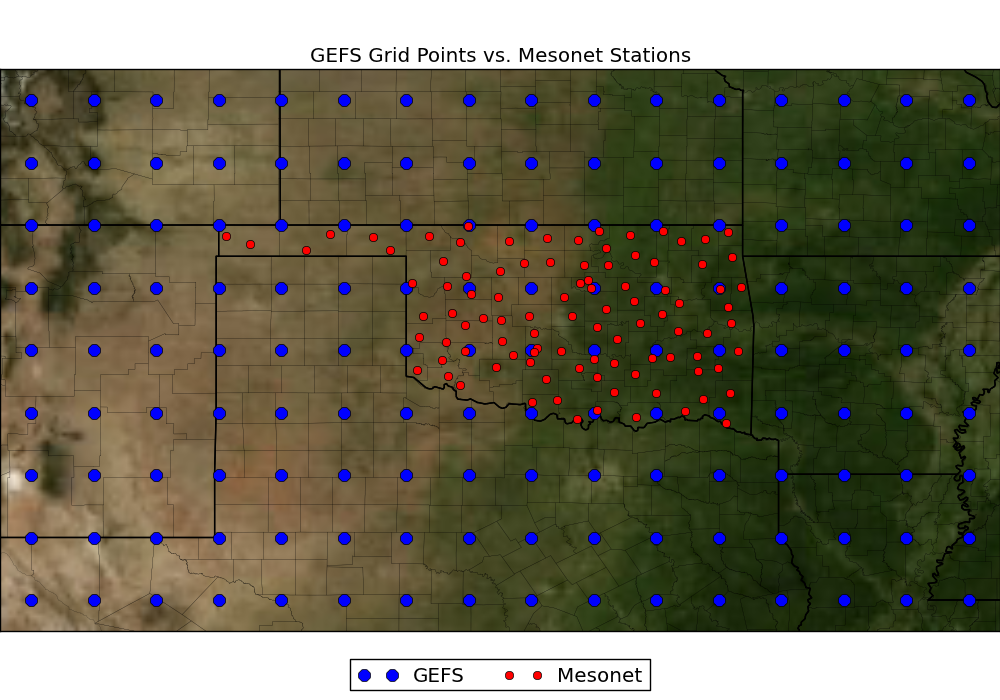
\includegraphics[width=\textwidth]{images/gefs_mesonet_stations.png}\\
    \begin{right}
    {\tiny{Courtesey: Dr. Amy}}
    \end{right}
  \end{figure}

    \end{column}
  \end{columns}

\begin{block}{Numerical weather prediction}
\begin{itemize}
     \item NOAA/NCEP GEFS Reforecast, 5 forecasts per day
     \item Ensemble comprises 11 members (one control)
     \item 15 variables (temp, humidity, upward radiative flux, ...)
  \end{itemize}
\end{block}

\end{frame}


% Slide 3 =====================================================================

\begin{frame}{Overview of our approach}

\end{frame}


% Slide 4 =====================================================================

\begin{frame}{Kriging}

\end{frame}


% Slide 5 =====================================================================

\begin{frame}{Feature engineering}

\end{frame}


% Slide 6 =====================================================================

\begin{frame}{Predicting energy production}

\end{frame}


% Slide 7 =====================================================================

\begin{frame}{Results}

\end{frame}



\end{document}
